%Dokumentinformationen
\newcommand{\titleinfo}{Analysis 2E - Formelsammlung}
\newcommand{\authorinfo}{F. Braun, L. Schmid, U. Giger, R. Koller, E. Ammann, S.
Arnold}
\newcommand{\versioninfo}{$Revision: 813 $ - powered by \LaTeX}

% standard header

%Dokumentinformationen
\newcommand{\titleinfo}{Analysis 2E - Formelsammlung}
\newcommand{\authorinfo}{KKK K\"oppel, K\"oppel und Konsortium, basierend auf
Sammlung von F. Braun \& Co}
\newcommand{\versioninfo}{$Revision: 2.0 $}



%%%%%%%%%%%%%%%%%%%%%%%%%%%%%%%%%%%%%%%%%%%%%%%%%%%%%%%%%%%%%%%%%%%%%%%%%%%%%%%%%%%%%%%%%%%%%%%%
% Neue Befehle und Definitionen                
%%%%%%%%%%%%%%%%%%%%%%%%%%%%%%%%%%%%%%%%%%%%%%%%%%%%%%%%%%%%%%%%%%%%%%%%%%%%%%%%%%%%%%%%%%%%%%%

\newcommand{\formelbuch}[1]{$_{\textcolor{red}{\mbox{\small{S#1}}}}$}
\newcommand{\verweis}[2]{\small{(siehe auch \ref{#1}, #2 (S. \pageref{#1}))}}
\newcommand{\subsubadd}[1]{\textcolor{black}{\mbox{#1}}}




%Schriftgr�sse, Layout, Papierformat, Art des Dokumentes
\documentclass[10pt,twoside,a4paper,fleqn]{article}
%Einstellungen der Seitenr�nder
\usepackage[left=1cm,right=1cm,top=1cm,bottom=1cm,includeheadfoot]{geometry}
% Sprache, Zeichensatz, packages
\usepackage[latin1]{inputenc}
\usepackage[ngerman]{babel,varioref}
\usepackage{amssymb,amsmath,fancybox,graphicx,color,lastpage,wrapfig,fancyhdr,hyperref,verbatim}

%Teile des Dokuments Mehrspaltig
\usepackage{multicol}
%Rotieren von Elementen (Bilder, Tabellen...)
\usepackage{rotating}

%Fliesstext
\usepackage{wrapfig}

%pdf info
\hypersetup{pdfauthor={\authorinfo},pdftitle={\titleinfo},colorlinks=false}
%linkbordercolor=white
\author{\authorinfo}
\title{\titleinfo}

%Kopf- und Fusszeile
\pagestyle{fancy}
\fancyhf{}
%Linien oben und unten
\renewcommand{\headrulewidth}{0.5pt} 
\renewcommand{\footrulewidth}{0.5pt}

\fancyhead[L]{\titleinfo{ }\tiny{(\versioninfo)}}
%Kopfzeile rechts bzw. aussen
\fancyhead[R]{Seite \thepage { }von \pageref{LastPage}}
%Fusszeile links bzw. innen
\fancyfoot[L]{\footnotesize{\authorinfo}}
%Fusszeile rechts bzw. ausen
\fancyfoot[R]{\footnotesize{\today}}

\definecolor{black}{rgb}{0,0,0}
\definecolor{red}{rgb}{1,0,0}
\definecolor{white}{rgb}{1,1,1}
\definecolor{grey}{rgb}{0.8,0.8,0.8} % ./header.tex nicht editieren (Projekt LaTeX-Header benutzen)

%%%%%%%%%%%%%%%%%%%%%%%%%%%%%%%%%%%%%%%%%%%%%%%%%%%%%%%%%%%%%%%%%%%%%%%%%%%%%%%%%%%%%%%%%%%%%%%%
% Neue Befehle und Definitionen                
%%%%%%%%%%%%%%%%%%%%%%%%%%%%%%%%%%%%%%%%%%%%%%%%%%%%%%%%%%%%%%%%%%%%%%%%%%%%%%%%%%%%%%%%%%%%%%%
\definecolor{black}{rgb}{0,0,0}
\definecolor{red}{rgb}{1,0,0}
\definecolor{white}{rgb}{1,1,1}
\definecolor{grey}{rgb}{0.8,0.8,0.8}
\newcommand{\formelbuch}[1]{$_{\textcolor{red}{\mbox{\small{S#1}}}}$}
\newcommand{\verweis}[2]{\small{(siehe auch \ref{#1}, #2 (S. \pageref{#1}))}}
\newcommand{\subsubadd}[1]{\textcolor{black}{\mbox{#1}}}

\begin{document}

\setlength{\parindent}{0pt}
           
%%%%%%%%%%%%%%%%%%%%%%%%%%%%%%%%%%%%%%%%%%%%%%%%%%%%%%%%%%%%%%%%%%%%%%%%%%%%%%%%%%%%%%%%%%%%%%%%
%%%%%%%%%%%%%%%%%%%%%%%%%%%%%%%%%%%%%%%%%%%%%%%%%%%%%%%%%%%%%%%%%%%%%%%%%%%%%%%%%%%%%%%%%%%%%%%%
\section{Integralrechnung \formelbuch{444}}
\subsection{Integrationsmethoden \formelbuch{447ff}}
	\begin{tabbing}
       xxxxxxxxxxxxxxxxxxxxxxxxxxxxxxx \= xxx \= xxxxxxxxxxxxxxxxxxxxxxxxxxxxxxxxxxxxxxxxxxxxxxxxxxxxxxx\kill  
       Linearität\>		  
 	   $\qquad\int{f(\alpha x+\beta )dx=\frac{1}{\alpha}\cdot F(\alpha x+
		\beta)+C}$\\ \\
  	   Partielle Integration\>
 	   $\qquad\int\limits_a^b{u'(x)\cdot v(x)dx}=\biggl[ u(x)\cdot v(x) \biggr]_a^b
 	   -\int\limits_a^b{u(x)\cdot v'(x)dx}$\\ \\ Substitution (Rationalisierung)\>
 	   $\qquad t=\tan\frac{x}{2}, \qquad dx=\frac{2dt}{1+t^2} \qquad 
 	   \sin  x=\frac{2t}{1+t^2} \qquad \cos x=\frac{1-t^2}{1+t^2}
		\quad\int{R(\sin(x)\cos(x))dx}$\\ 
 	   Allgemeine Substitution \> \>
		$\int\limits_{a}^{b}{f(x)dx}=\int\limits_{g^{-1}(a)}^{g^{-1}(b)}{f(g(t))\cdot
		g'(t)dt}\qquad t=g^{-1}(x)\qquad  \fbox{x=g(t)}\qquad dx=g'(t)\cdot dt$\\
 	   Logarithmische Integration \>\>
 	    $ \int{\frac{f'(x)}{f(x)}dx}=\ln|f(x)|+C	\qquad{(f(x)\neq 1)}$\\ \\
	   Spezielle Form des Integranden \>\>
 		$\int{f'(x)\cdot (f(x))^{\alpha} dx}= f(x)^{\alpha +1}\cdot
 		\frac{1}{\alpha+1}+C \qquad{(\alpha \neq -1)}$\\ 
 	   Differentiation\>\>
 		$\int \limits ^{b} _{a} {f'(t)dt}=f(b)-f(a)$\\ \>\>
		$\frac{d}{dx} \int \limits ^{x} _{1} {f(t)dt}=f(x)$
    \end{tabbing}

\subsubsection{Einige unbestimmte Integrale \formelbuch{1053 ff}}
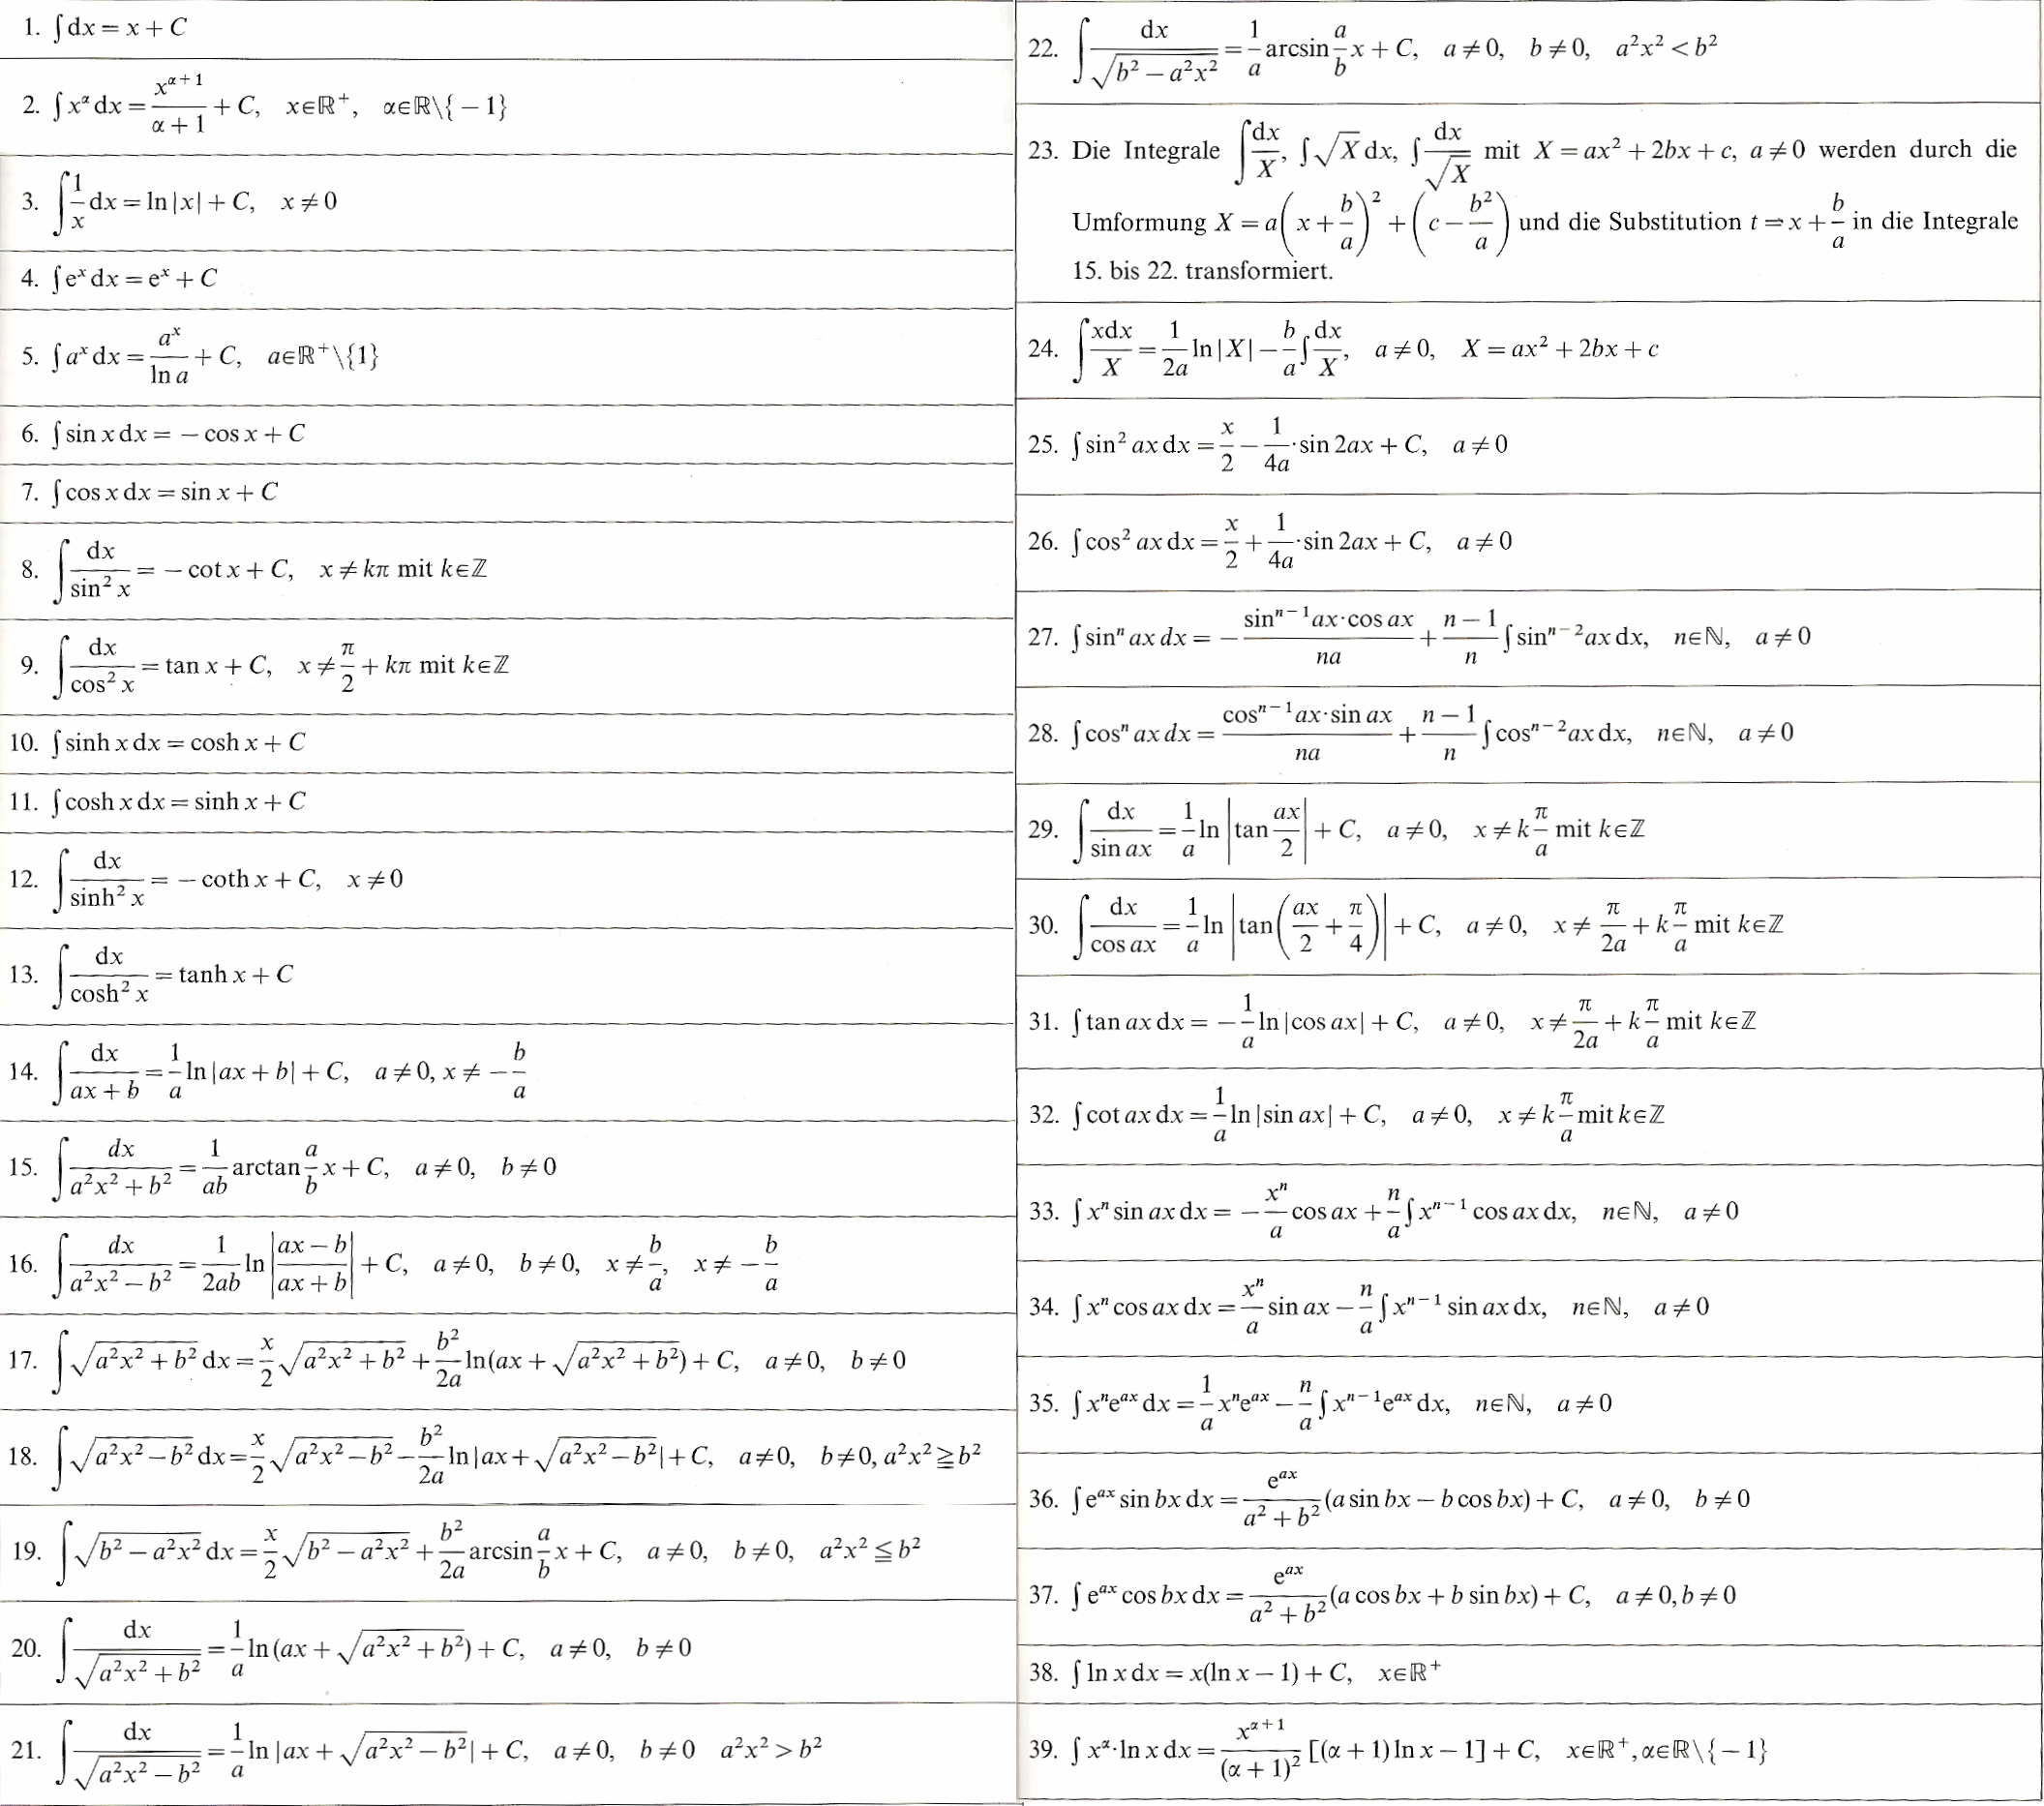
\includegraphics[width=17.7cm]{./bilder/integrale.png} 

\subsection{Uneigentliche Integrale}
	Uneigentliches Integral heisst, dass entweder eine \textbf{unbeschränkte
	Funktion} integriert wird, oder eine Funktion über einen \textbf{unbeschränkten Integrationsberech} 
	integriert wird.$\\$
	\begin{minipage}{100mm}
    
	Für unbeschränkte Funktionen:$\\$
	$I =\int\limits _{a}^{c}f(x)dx=
	\lim\limits_{t\to 
	b-}\int\limits_{a}^{t}f(x)dx+\lim\limits_{t\to b+}\int\limits_{t}^{c}f(x)dx\\
	\\$ Für die unbeschränkte Integration:$\\$
	$I =\int\limits _{a} ^{\infty} f(x)dx= \lim \limits_{t\to \infty}\int \limits
	_{a} ^{t}f(x)dx;\\$
	$I =\int\limits ^{a} _{-\infty} f(x)dx= \lim \limits_{t\to -\infty}\int
	\limits _{t} ^{a}f(x)dx; \\$
	$I =\int\limits _{-\infty} ^{\infty} f(x)dx = \lim \limits_{t_1\to \infty} \lim
	\limits
	_{t_2 \to  \infty}\int \limits _{t_1} ^{a}f(x)dx + \int\limits_{a}^{t_2}f(x)dx\\$
	Beispiel: $\int\limits_{1}^{\infty}\frac{1}{x^2}dx=\lim\limits_{t\to \infty}\int\limits_{1}^{t}\frac{1}{x^2}dx=\lim\limits_{t\to \infty}-\frac{1}{t}+\frac{1}{1}=1$
    \end{minipage}
	\begin{minipage}{100mm}
    	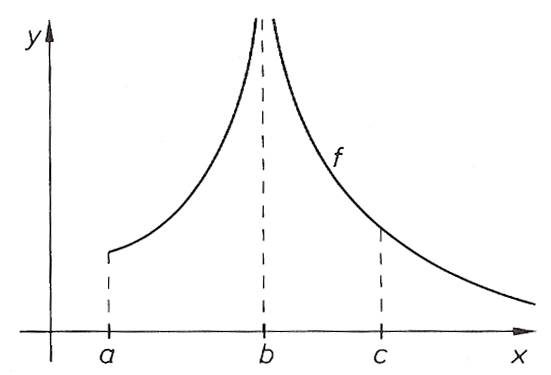
\includegraphics[width=3cm]{./bilder/unbeschraenkteFunktion.png} $\\$
    	unbeschränkte Funktion
    \end{minipage}
\subsubsection{Prinzip der Restfläche}
	Wenn $\lim\limits_{t \rightarrow \infty} \int\limits^{\infty}_{t} f(x) dx = 0$, dann konvergiert
	$\int\limits_a^{\infty} f(x) dx$ und umgekehrt.

\subsubsection{Majorantenprinzip}
	Um nachzuweisen, ob eine Funktion $|f(x)| \geq 0$ konvergiert, wird eine zweite
	Funktion $g(x) \geq |f(x)|$ (Majorante) gesucht. Konvergiert $\int\limits_a^{\infty} g(x) dx$,
	dann konvergiert auch $\int\limits_a^{\infty} f(x) dx$. ($x \in [a, \infty)$)

\subsubsection{Minorantenprinzip}
	Um nachzuweisen, ob eine Funktion $f(x)$ divergiert, wird eine zweite
	Funktion $0 \leq g(x) \leq f(x)$ (Minorante) gesucht. Divergiert
	$\int\limits_a^{\infty} g(x) dx$,
	dann divergiert auch $\int\limits_a^{\infty} f(x) dx$. ($x \in [a, \infty)$)
	
\section{Funktionsgraphen}
\begin{tabular}{lll}
\parbox{5.5cm}{
	\textbf{e-Funktion} \\
	%%$$e^x=\lim_{n \to \infty} (1+\frac{x}{n})^n$$				
	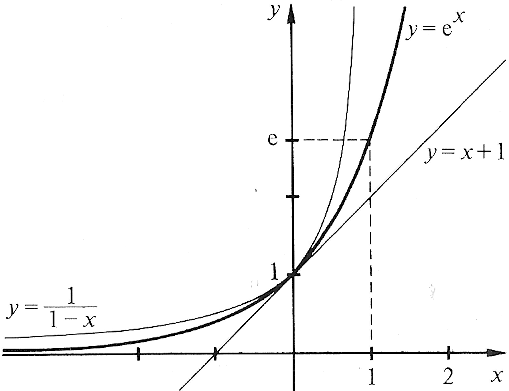
\includegraphics[width=4.5cm]{./bilder/funktionen_e.png} \\ \\
	
	\textbf{Logarithmus-Funktion}\\
	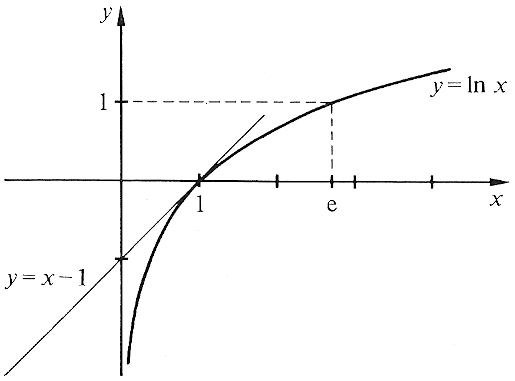
\includegraphics[width=4.5cm]{./bilder/funktionen_ln.png} 
}
& \parbox{5.5cm}{
	\textbf{Trigonometrische Funktionen}\\
	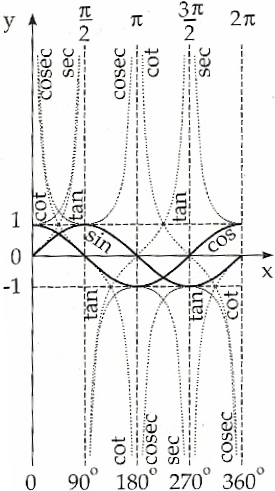
\includegraphics[width=4.5cm]{./bilder/funktionen_trigo.png} 
}
& \parbox{7cm}{
	\textbf{Hyperbel Funktionen}\\
	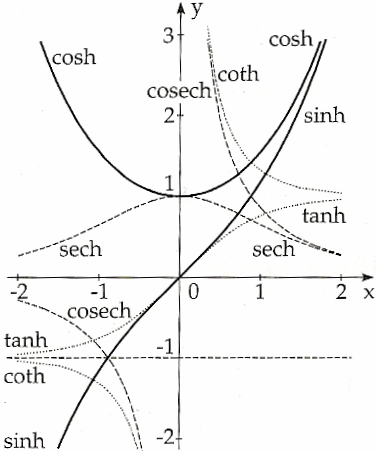
\includegraphics[width=6cm]{./bilder/funktionen_hyperbel.png} 
}
\end{tabular}

%%%%%%%%%%%%%%%%%%%%%%%%%%%%%%%%%%%%%%%%%%%%%%%%%%%%%%%%%%%%%%%%%%%%%%%%%%%%%%%%%%%%%%%%%%%%%%%%
%%%%%%%%%%%%%%%%%%%%%%%%%%%%%%%%%%%%%%%%%%%%%%%%%%%%%%%%%%%%%%%%%%%%%%%%%%%%%%%%%%%%%%%%%%%%%%%%
\newpage
\section{Anwendung der Differential- und Integralrechnung}

\subsection{Beschreibungungsvarianten}
	\begin{minipage}[t]{3.5cm}
		Funktion (explizit) \\
		$ y = f(x)$ \\
        \tiny{(Bronstein Form 3.425)}
	\end{minipage}
	\begin{minipage}[t]{6cm} 		
		Koordinatengleichung (implizit) \\
		$ F(x,y) = 0 $ \\
        \tiny{(Bronstein Form 3.424)}
	\end{minipage}
	\begin{minipage}[t]{5.5cm} 		
		Parameterform \\
		$ \left( \begin{array} {l} x(t) \\ y(t) \end{array} \right) =
          \left( \begin{array} {l} \Psi(t) \\ \varphi(t) \end{array} \right)$\\
        \tiny{(Bronstein Form 3.426)}
	\end{minipage} 
	\begin{minipage}[t]{3cm}
    	Polarform x\\
    	$ r=f(\varphi) $ \\
        \tiny{(Bronstein Form 3.427)}
    \end{minipage}\\

	\textit{Hat man die explizite Form gegeben, so hat man automatisch die
	Implizite- und Parameter-Form}

\subsection{Umrechnen diverser Systeme \formelbuch{(196)}}
\begin{tabular}{lll}
Parameter 
	& $\Rightarrow$ explizit
	%& $x = f(t) \; \; y = g(t)$
	& $\Longrightarrow t = f(x);\; y = g(f(x))$\\
Ex- bzw. implizit 
	& $\Rightarrow$ Polar
	%& $y = f_1(x)$ bzw. $f_2(x,y) = C$
	& $\Longrightarrow$ Ersetze $x$ durch $r
\cos(\varphi)$ \& $y$ durch $r \sin(\varphi)$\\ 
Polar 
	& $\Rightarrow$ implizit
	%& $r = f(\varphi)$
	& $\Longrightarrow$ Ersetze $r \sin(\varphi)$ durch $y$, $r \cos(\varphi$ durch
	$x$, $r$ durch $\sqrt{x^2 + y^2}$\\ 
Polar
	& $\Rightarrow$ Parameterform
	%& $r = f(\varphi)$
	& $\Longrightarrow \left( \begin{array} {l} x(\varphi) \\ y(\varphi) \end{array} \right) =
          \left( \begin{array} {l} r(\varphi) \cos(\varphi) \\ r(\varphi) \sin(\varphi) \end{array}
          \right)$ \\
Explizit
	& $\Rightarrow$ Parameter
	%& $y = f(x)$
	& $\Longrightarrow \left( \begin{array} {l} x(t) \\ y(t) \end{array} \right) =
          \left( \begin{array} {l} x(t)) \\ t \end{array}
          \right)$ \\
Einzelner Punkt  
	& $\Rightarrow$ Polar
	%& $(x,\; y)$
	& $\Longrightarrow r = \sqrt{x^2 + y^2};\;
	\varphi = \begin{cases}\arctan(\frac{y}{x}) + \pi 	&x < 0\\
             \arctan(\frac{y}{x}) 	& x > 0\\
             \frac{\pi}{2}			& x = 0;\; y > 0\\
             -\frac{\pi}{2}			& x = 0;\; y < 0\\
             \text{unbestimmt}		& x = y = 0\end{cases}$\\
\end{tabular}

\subsection{Kurvenarten\formelbuch{202ff}}
\begin{tabular}{llll}
\parbox{2.7cm}{
\textbf{ } \\
Implizit:\\
Bemerkung:\\
Polarform:\\
Parameterform:
}

\parbox{6cm}{
\textbf{Kreis\formelbuch{202}}\\
$(x-x_0)^2 + (y - y_0)^2 = r^2$\\
Mittelpunkt $(x_0, y_0)$; Radius $r$\\
$r = \frac{p}{1 + \epsilon \cos(\varphi)}; \epsilon = 0$ \\
$x=x_0 + R\cos(t), y=y_0 + R\sin(t)$
}

\parbox{8cm}{
\textbf{Ellipse\formelbuch{204}}\\
$(\frac{x-x_0}{a})^2 + (\frac{y-y_0}{b})^2 = 1$\\
Mittelpunkt $(x_0, y_0)$; Halbachsen $a$, $b$\\
$r = \frac{p}{1 + \epsilon \cos(\varphi)}; 0 < \epsilon < 1$\\
$x = a\cos(t), y = b\sin(t)$
}\\ \\

\parbox{2.7cm}{
\textbf {}\\
Implizit:\\
Bemerkung:\\
Polarform:\\
Parameterhform:
}

\parbox{6cm}{
\textbf{Hyperbel\formelbuch{206}}\\ 
$(\frac{x}{a})^2 - (\frac{y}{b})^2 = 1; -(\frac{x}{a})^2 + (\frac{y}{b})^2 =1$\\ 
\\
$r = \frac{p}{1 + \epsilon \cos(\varphi)}; \epsilon > 1$\\
$x= a \cosh(t), y = b \sinh(t) $
}

\parbox{8cm}{
\textbf{Parabel\formelbuch{209}}\\
$y= ax^2 + bx + c$\\
Parabeln mit Scheitelpunkt auf der vertikaler Achse\\
$r = \frac{p}{1 + \epsilon \cos(\varphi)}; \epsilon = 1$\\
$x=t, y = a t^2 + b t + c$
}\\ \\

\parbox{2.7cm}{
\textbf{} \\
Polarform:
}

\parbox{5cm}{
\textbf{Kardioide/Herzk. \formelbuch{99}} \\
$r = a(1+\cos(\varphi))$
}

\parbox{5cm}{
\textbf{Lemniskate ``$\infty$'' \formelbuch{101}} \\
$r = a\sqrt{2\cos(2\varphi)}$ 
}

\parbox{5cm}{
\textbf{Strophoide/harm. K. \formelbuch{96}} \\
$ r = -a \frac{\cos(2\varphi)}{\cos(\varphi)},(a>0) $ 
}

\end{tabular}

\subsection{Gleichungen\formelbuch{234}, Mittelwerte\formelbuch{19ff}}
\begin{tabular}{llll}
	\textbf{Tangentengleichung} &
	\textbf{Normalengleichung} &
	\textbf{Linearer Mittelwert} &
	\textbf{Quadratischer Mittelwert}\\
	$y-y_0=f'(x_0)(x-x_0)$ &
	$y-y_0=-\frac{1}{f'(x_0)}(x-x_0)$ &
	$\bar{f} = \frac{1}{b-a} \int\limits_{a}^{b} f(x)dx$ &
	$\bar{f} = \sqrt{\frac{1}{b-a} \int\limits_{a}^{b} f(x)^2dx}$
\end{tabular}
	
\subsection{Tangenten- \& Normalenabschnitt, Subtangente \& Subnormale\formelbuch{234ff}}

\subsection{Abstandsformeln}
\begin{minipage}{6.5cm}
    \textbf{Hessesche Normalform\formelbuch{200f, 221}}\\
    $x\cdot \cos\varphi_0 +y\cdot \sin\varphi_0=r_0$\\
    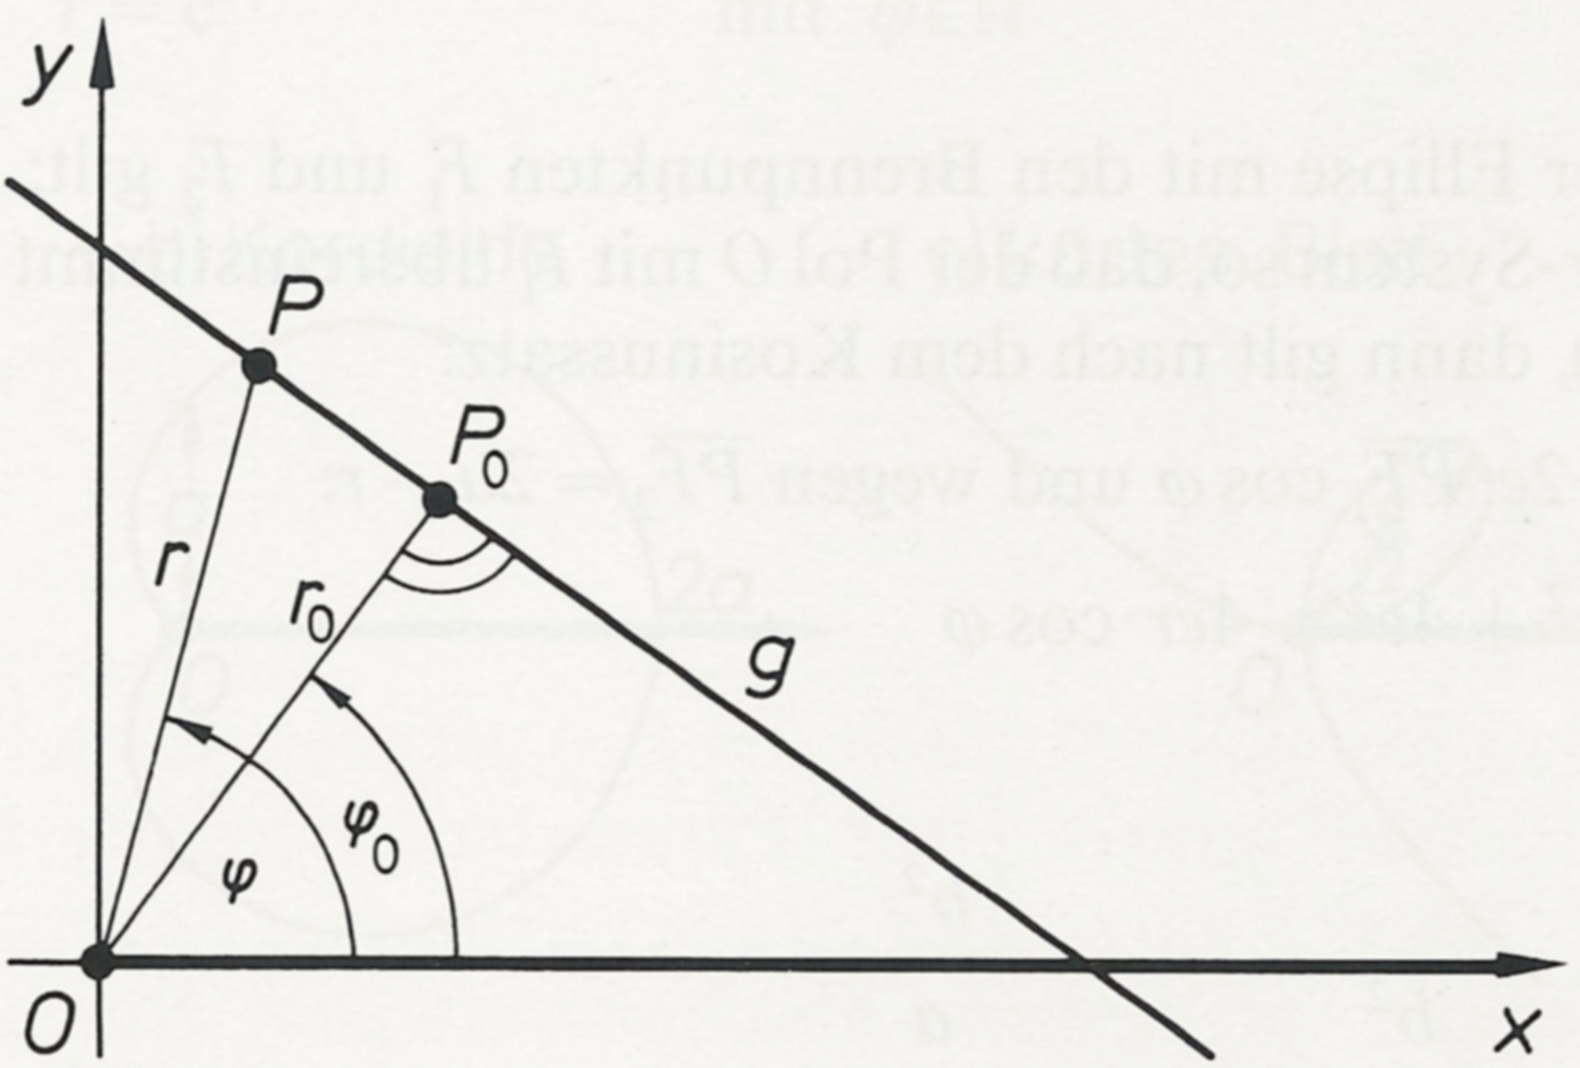
\includegraphics[width=2.8cm]{./bilder/hessenorm.png}
\end{minipage}
\begin{minipage}{6.5cm}
	\textbf{Geradengleichung} \\
	$y - y_0 = m (x - x_0)$
\end{minipage}
\begin{minipage}{6cm}
	\textbf{Abstand zum Ursprung} \\
	$\frac{|y_0 - m \cdot x_0|}{\sqrt{m^2 + 1}}$
\end{minipage}

\subsection{Berührung höherer Ordnung}
Zwei explizit gegebene Kurven $y = f(x)$ und $y = g(x)$ berühren einander im
Punkt P $x_0, y_0$ von der Ordnung $n$, wenn die Funktionswerte und die ersten
$n$ Ableitungen existieren und übereinstimmen.\\
$f(x_0) = g(x_0);\; f'(x_0) = g'(x_0);\; f''(x_0) = g''(x_0);\;\ldots ;
\;f^{(n)}(x_0) = g^{(n)}(x_0)\; \qquad f^{(n+1)}(x_0) \neq g^{(n+1)}(x_0)$

\subsection{Scheitel \formelbuch{339}}
Scheitelpunte sind Extremalwerte der Krümmungs- bzw. Krümmungsradiusfunktion.
Falls bei $\kappa'(x)$ an der Stelle $x_0$ ein Vorzeichenwechsel besteht, existiert dort
eine Extremalstelle. 

\subsection{Wichtige Formeln\formelbuch{232ff}}
	\renewcommand{\arraystretch}{2}
	\begin{tabular}[c]{ | p{5.1cm} | p{5.4cm} | l | }
		\hline
		\textbf{Cartesisch} & \textbf{Parameter} & \textbf{Polar} \\
		\hline
		\multicolumn{3}{| l |}{\textbf{Anstieg einer Kurve, Ableitung, 2. Ableitung}} \\
    	\hline   
    	$y'=f'(x_o) \quad y'' = f''(x_0)$ & 
    	$y'=\frac{\dot{y}}{\dot{x}} \quad 
    	y'' = \frac{\dot{x} \ddot{y} - \dot{y}\ddot{x}}{\dot{x}^3}$ &
    	$y'=\frac{r'(\varphi) \sin(\varphi) + r(\varphi) \cdot
    	\cos(\varphi)}{r'(\varphi) \cos(\varphi)-r(\varphi) \cdot \sin(\varphi)}$
    	\\
		
		\hline
		\multicolumn{3}{| l |}{\textbf{Bogenlänge \formelbuch{233, 466}}} \\
    	\hline
    	$s=\int\limits_a^b{\sqrt{1+(f'(x))^2}dx}$ & 
    	$|s|=\int\limits_{t_1}^{t_2}{\sqrt{\dot{x}^2(t)+\dot{y}^2(t)}dt}$ &
		$|s|=\int\limits_{\varphi_1}^{\varphi_2}{\sqrt{(r'(\varphi))^2+((\varphi))^2}d\varphi}$\\
		
		\hline		
		\multicolumn{3}{| l |}{\textbf{Krümmung ebener Kurven \formelbuch{236}}}\\
    	\hline
    	$\kappa=\frac{f''(x)}{(\sqrt{1+(f'(x))^2})^3}$ &
    	$\kappa=\frac{\dot{x}(t)\ddot{y}(t)-\dot{y}(t)\ddot{x}(t)}{(\sqrt{(\dot{x}(t))^2+(\dot{y}(t))^2})^3}$ &
		$\kappa=\frac{2(r'(\varphi))^2-r(\varphi)r''(\varphi)+(r(\varphi))^2}{(\sqrt{(r'(\varphi))^2+(r(\varphi))^2})^3}$\\   	
		
		\hline
		\multicolumn{3}{| l |}{Konvex (Linkskurve): $\kappa \geq 0 \qquad$ Streng
		konvex: $\kappa > 0 \qquad$ Wendepunkt: $\kappa = 0 \qquad$ Analog für konkav}\\
		
		\hline
		\multicolumn{3}{| l |}{\textbf{Krümmungskreisradius \formelbuch{236f}}} \\
		\hline
		$r = \left|\frac{(\sqrt{1+(f'(x))^2})^3}{f''(x)} \right|$ &
		$r = \left|\frac{(\sqrt{(\dot{x}(t))^2+(\dot{y}(t))^2})^3}
		{\dot{x}(t)\ddot{y}(t)-\dot{y}(t)\ddot{x}(t)} \right|$ & 
		$r = \left|\frac{(\sqrt{(r'(\varphi))^2+(r(\varphi))^2})^3}
		{2(r'(\varphi))^2-r(\varphi)r''(\varphi)+(r(\varphi))^2} \right|$ \\
		
		\hline		
		\multicolumn{3}{| l |}{\textbf{Flächeninhalt \formelbuch{465}}} \\
    	\hline
    	$A=\int\limits_a^b{f(x)}dx$  & 
    	$A=\frac{1}{2}\int\limits_{t_1}^{t_2}{[x(t)\dot{y}(t)-\dot{x}(t)y(t)]dt}$ &
		$A=\frac{1}{2}\int\limits_{\varphi_1}^{\varphi_2}{(r(\varphi))^2d\varphi}$\\  
    	
		\hline		
		\multicolumn{3}{| l |}{\textbf{Volumen \formelbuch{467}}} \\
    	\hline
		$V=\pi\int\limits_a^b(f(x))^2dx$ & 
    	$V=\pi\left|\int\limits_{t_1}^{t_2}{(y(t))^2\dot{x}(t)dt}\right|$ &
		$V=\pi\left|\int\limits_{\varphi_1}^{\varphi_2}{r^2(\varphi)\sin^2\varphi[r'(\varphi)\cos(\varphi)-r(\varphi)\sin(\varphi)]d\varphi}\right|$\\  
    	
		\hline		
		\multicolumn{3}{| l |}{\textbf{Oberflächeninhalt \formelbuch{466f}}} \\
    	\hline
   		$O=2\pi\int\limits_a^b{|f(x)|\sqrt{1+(f'(x))^2}dx}$ & 
    	$O=2\pi\int\limits_{t_1}^{t_2}{|y(t)|\sqrt{\dot{x}^2(t)+(\dot{y}^2(t))}dt}$ &
		$O=2\pi\int\limits_{\varphi_1}^{\varphi_2}{|r(\varphi)\sin\varphi|\sqrt{(r'(\varphi))^2+(r(\varphi))^2}d\varphi}$\\  
    	\hline
	\end{tabular}
	\renewcommand{\arraystretch}{1}
\subsection{Orthogonaltrajektorien}
\begin{tabular}{ll}
\parbox{4.5cm}{
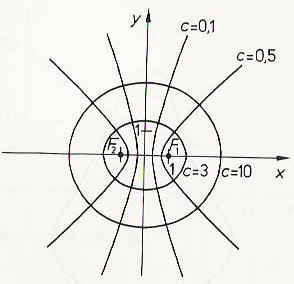
\includegraphics[height=4cm]{./bilder/orthoTrajekt.png}
}
& \parbox{14.5cm}{
Die orthogonalen Trajektorien schneiden alle Kurven der gegebenen Kurvenschar
$y=f(x,c)$ im rechten Winkel.\\
Die DGL $F(x,y,y')$ der Kurve bestimmen, anschliessend $y'$ durch
$-\frac{1}{y'}$ ersetzen.\\
$\Rightarrow$ ergibt die DGL der orthogonalen Trajektorien.\\
 \\
Die Kreise sind Orthogonaltrajektorien der Hyperbeln und umgekehrt.
}
\end{tabular}

%%%%%%%%%%%%%%%%%%%%%%%%%%%%%%%%%%%%%%%%%%%%%%%%%%%%%%%%%%%%%%%%%%%%%%%%%%%%%%%%%%%%%%%%%%%%%%%%
%%%%%%%%%%%%%%%%%%%%%%%%%%%%%%%%%%%%%%%%%%%%%%%%%%%%%%%%%%%%%%%%%%%%%%%%%%%%%%%%%%%%%%%%%%%%%%%%
\newpage
\section{Reihen\formelbuch{420, 427, 1045}}

\subsection{Zahlenreihen\formelbuch{422}}
$ s_n = \sum\limits_{k=1}^{n} a_k \qquad $ ist eine (unendliche) Reihe. Sie ist die Folge von Partialsummen einer bestehenden Folge $a_n$.

\subsubsection{Konvergenz, Divergenz\formelbuch{422}}
Konvergiert die Reihe $< s_n >$ gegen die Summe $ s = \sum\limits_{k=1}^{\infty} a_k $ so ist sie konvergent. 
Existiert der GW nicht, so ist sie divergent.

\subsubsection{Konvergenzkriterien}

\paragraph{Cauchy-Kriterium} 
Wenn zu jedem $\varepsilon > 0$ ein Index $n_0$ existiert, so dass für alle $m > n > n_0$ gilt: \\
$\left| \sum\limits_{k=n}^m a_k \right| < \varepsilon$, dann konvergiert die Reihe, ansonsten divergiert sie.

\paragraph{lim = 0\formelbuch{423}}
Wenn die Reihe $ \sum\limits_{n=1}^{\infty} a_n $ konvergent ist, so ist $\lim\limits_{n \to \infty} a_n = 0$. \hspace{2cm} Aber NICHT UMGEKEHRT!

\paragraph{Divergenz}
Ist $<a_n>$ divergent oder ist $\lim\limits_{n \to \infty} a_n \neq 0$, so ist die Reihe $ \sum\limits_{n=1}^{\infty} a_n $ divergent.

\paragraph{Majorantenkriterium\formelbuch{429}}
Ist die Reihe $ \sum\limits_{n=1}^{\infty} c_n $ konvergent, so konvergiert auch die Reihe $ \sum\limits_{n=1}^{\infty} a_n $ für $|a_n| \leq c_n$ (absolut). \\
Dies gilt auch für $|a_n| \leq c_n$ erst ab einer Stelle $n_0 \in \mathbb{N}$.

\paragraph{Minorantenkriterium}
Ist die Reihe $ \sum\limits_{n=1}^{\infty} d_n $ gegen $+\infty$ divergent, so gilt dies auch für die Reihe $ \sum\limits_{n=1}^{\infty} a_n $ 
bei $a_n \geq d_n$. \\ Dies gilt auch für $a_n \geq d_n$ erst ab einer Stelle $n_0 \in \mathbb{N}$.

\paragraph{Reziprokkriterium}
$ s = \sum\limits_{n=1}^{\infty} \frac{1}{n^\alpha} $ ist konvergent für $\alpha > 1$ und divergent für $\alpha \leq 1$.

\paragraph{Quotientenkriterium\formelbuch{424}}
$ \lim\limits_{n \to \infty} \left|\frac{a_{n+1}}{a_n}\right| = \alpha $ der Reihe $ \sum\limits_{n=1}^{\infty} a_n $ \\
$\alpha < 1 \Rightarrow$ (absolut) konvergent \hspace{3cm}
$\alpha > 1 \Rightarrow$ divergent \hspace{4cm} 
$\alpha = 1 \Rightarrow$ keine Aussage!

\paragraph{Wurzelkriterium\formelbuch{424f}}
$ \lim\limits_{n \to \infty} \sqrt[n]{\left|a_n\right|} = \alpha $ der Reihe $ \sum\limits_{n=1}^{\infty} a_n $ \\
$\alpha < 1 \Rightarrow$ (absolut) konvergent\hspace{3cm}
$\alpha > 1 \Rightarrow$ divergent \hspace{4cm} 
$\alpha = 1 \Rightarrow$ keine Aussage!

\paragraph{Integralkriterium\formelbuch{425}}
$ \sum\limits_{n=1}^{\infty} f(n) $ ist konvergent, wenn das uneigentliche Integral $ \int\limits_{1}^{\infty} f(x) dx $ konvergent ist. \\
Gilt nur, wenn $f$ auf $ [1, \infty) $ definiert und monoton fallend ist. Zudem muss $ f(x) \geq 0 $ für alle $x \in [1, \infty)$ sein.
 
\paragraph{Leibniz-Kriterium\formelbuch{426}}
Die \textbf{alternierende} Reihe $ \sum\limits_{n=1}^{\infty} a_n $ ist konvergent, wenn die Folge $<\left|a_n\right|>$ eine monoton fallende Nullfolge ($\lim\limits_{n \to \infty}
\left|a_n\right| = 0 $) ist.
\\ Monotonie mittels Verhältnis ($ \left|\frac{a_{n+1}}{a_n}\right| $), Differenz ($ |a_{n+1}| - |a_n| $) oder \textit{vollständiger Induktion} beweisen.\\ 

\paragraph{Abschätzung Restglied einer alternierenden konvergenten Reihe\formelbuch{426,430}}\qquad $|R_n| = |s-s_n|\leq |a_{n+1}|$


\subsubsection{Bedingte und Absolute Konvergenz\formelbuch{425}}
Eine Reihe $\sum\limits_{n=1}^{\infty}a_n$ heisst \textbf{absolut konvergent}, wenn die
Reihe $\sum\limits_{n=1}^{\infty}|a_n|$ konvergent ist.\\
\textbf{Bedingt Konvergent:} Eine Reihe hat durch Umordnen einen anderen
Grenzwert oder wird divergent.\\
\textbf{Unbedingt Konvergent:} Durch Umordnen ändert sich der Grenzwert nicht.

\subsubsection{Produkt von absolut konvergenten Reihen\formelbuch{426}} 
Gegeben sei: $\sum a_n=a$, \quad $\sum b_n=b, \quad \sum c_n = (\sum a_n) \cdot (\sum b_n) = c \quad $ so ist
$ \quad c_n=\sum a_kb_{n-k+1} \quad $ und $ \quad c = a \cdot b $



\subsection{Potenzreihen}

\paragraph{Definition\formelbuch{432}} 
Die Reihe $ \sum\limits_{n=0}^{\infty} a_n (x-x_0)^n $ heisst Potenzreihe mit Entwicklungspunkt $x_0$ und Koeffizienten $a_n$.

\begin{tabular}{lll}
\textbf{Geometrische Reihe\formelbuch{19}}
	& $ \frac{a}{1-x} = a \cdot \sum\limits_{n=0}^{\infty} x^n$
	& $(|x| < 1) \qquad$ Beidseitiges $\int \quad\Rightarrow\quad -a \cdot \ln{|x-1|} 
= a \cdot \sum\limits_{n=1}^{\infty} \frac{x^{n}}{n} $ \\
\textbf{Binominalreihe} 
	& $ (1+x)^\alpha = \sum\limits_{n=0}^\infty \binom{\alpha}{n} x^n$
	& $x \in (-1,1)$ \\
\textbf{Taylor-Reihe\formelbuch{434, 1045}}
	& $ \sum\limits_{n=0}^{\infty} \frac{f^{(n)}(x_0)}{n!}\cdot(x-x_0)^n$
	& Taylor-Reihe von f bezüglich der Stelle $x_0$ \\
\textbf{E-Funktion}
	& \multicolumn{2}{l}{$e = \lim\limits_{n\to\infty} \left(1+\frac{1}{n}\right)^n = 
	\sum\limits_{k=0}^{\infty}{\frac{1}{k!}} = 1 + \frac{1}{1} + \frac{1}{1\cdot 2} +
	\frac{1}{1\cdot 2\cdot 3}  + \frac{1}{1\cdot 2\cdot 3\cdot4} + \cdots$}
\end{tabular}

\subsubsection{Konvergenz\formelbuch{432}}
Gegeben sei die Potenzreihe $ \sum\limits_{n=0}^{\infty} a_n x^n $ mit $ \lim\limits_{n \to \infty} \sqrt[n]{|a_n|} = a $ \\
Für $ a=0 $ ist die Potenzreihe für alle $ x \in \mathbb{R} $ absolut konvergent. \\
Für $ a>0 $ ist die Potenzreihe für alle $x$ mit 
$	\left\{ 	
		\begin{array}{l} 
			|x| < \frac{1}{a} = \rho \Rightarrow \text{ absolut konvergent.} \\
			|x| > \frac{1}{a} = \rho \Rightarrow \text{ divergent.}
		\end{array} 
	\right. $ \\
Ist die Folge $<\sqrt[n]{|a_n|}>$ nicht beschränkt, so ist die Potenzreihe nur für $x=0$ konvergent.

\subsubsection{Konvergenzradius\formelbuch{432}}
Jeder Potenzreihe kann ein Konvergenzradius $\rho$ zugeordnet werden. Wobei gilt $\rho = \frac{1}{a}$ mit $a = \lim\limits_{n \to \infty} \sqrt[n]{|a_n|} $. \\
Für $a = 0$ gilt $\rho = \infty$. Wenn a nicht exisitiert (Folge divergent) ist $\rho = 0$. \\
Berechnung mittels Quotientenkriterium: $ \rho = \lim\limits_{n \to \infty} \left| \frac{a_n}{a_{n+1}} \right|$

\subsubsection{Differentiation}
Alle Potenzreihen mit einem $\rho > 0$ sind für alle $x \in (-\rho, \rho)$ beliebig oft (gliedweise) differenzierbar. \\
Der Potenzradius $\rho$ ist bei allen Ableitungen gleich demjenigen der Ursprungsfunktion. $\rho_{f} = \rho_{f^{(i)}}$.
$$ f(x) = \sum\limits_{n=0}^{\infty} a_n x^n  \qquad 
   f'(x) = \sum\limits_{n=1}^{\infty} n \cdot a_n x^{n-1 } \qquad 
   f''(x) = \sum\limits_{n=2}^{\infty} n(n-1) \cdot a_n x^{n-2} \qquad 
   f^{(i)}(x) = \sum\limits_{n=i}^{\infty} n(n-1)\cdot \ldots \cdot (n-i+1)\cdot a_n x^{n-i} $$ 
\textbf{Bemerkung:} Startwert ($n=0$) nur erhöhen, wenn bei $x^n, n$ negativ werden würde!

\subsubsection{Integration}
\paragraph{Unbestimmtes Integral}
$\int \sum\limits_{n=0}^{\infty} a_n x^n dx = 
\sum\limits_{n=0}^{\infty} a_n \int x^n dx = 
\sum\limits_{n=0}^{\infty} \frac{a_n}{n+1}\cdot x^{n+1} \qquad \text{ für alle } x \in (-\rho, \rho).$
\paragraph{Bestimmtes Integral}
$\int\limits_0^x \sum\limits_{n=0}^{\infty} a_n t^n dt = 
\sum\limits_{n=0}^{\infty} \frac{a_n}{n+1}\cdot x^{n+1} \qquad \text{ für alle } x \in (-\rho, \rho).$


%%%%%%%%%%%%%%%%%%%%%%%%%%%%%%%%%%%%%%%%%%%%%%%%%%%%%%%%%%%%%%%%%%%%%%%%%%%%%%%%%%%%%%%%%%%%%%%%
%%%%%%%%%%%%%%%%%%%%%%%%%%%%%%%%%%%%%%%%%%%%%%%%%%%%%%%%%%%%%%%%%%%%%%%%%%%%%%%%%%%%%%%%%%%%%%%%

\newpage
\section{Differentialgleichungen}

\subsection{Lösen von Differentialgleichungen}

\subsubsection{Trennung von Variabeln \formelbuch{506}}
\begin{tabular}{p{4cm}p{1.5cm}p{10.5cm}}
\textbf{Form:} $y' = f(x) g(y)$ &
\textbf{Vorgehen:}              &
$\frac{y'}{g(y)} = f(x)$, nun ist die DGL beidseitig nach x integrierbar\\  &&
($dx = \frac{dy}{y'}$): $\int \frac{1}{g(y)} dy = \int f(x) dx$ 
\end{tabular}

\subsubsection{Lineartermsubstitution \formelbuch{506}}
\begin{tabular}{p{4cm}p{1.5cm}p{10.5cm}}
\textbf{Form:} $y'=f(ax+by+c)$   &
\textbf{Vorgehen:}               &
1. Substitution: $z=ax+by+c \qquad z'=a+by' =a+bf(z)$\\ &&
$\int\frac{z'}{a+bf(z)} = \int 1$
\end{tabular}

\subsubsection{Gleichgradigkeit}
\begin{tabular}{p{4cm}p{1.5cm}p{10.5cm}}
\textbf{Form:} $y'=f(\frac{y}{x})$ &
\textbf{Vorgehen:}                &
1. Substitution: $z=\frac{y}{x} \qquad
z'=\frac{1}{x}(f(z)-z)$
\end{tabular}

\subsubsection{Lineare Differentialgleichungen 1. Ordnung \formelbuch{507}}
\begin{tabular}{p{4cm}p{1.5cm}p{10.5cm}}
\textbf{Form:} $ y'+f(x)y = g(x) $ &
\textbf{Vorgehen:}                 &
$ y=e^{-\int f(x) dx}(k+\int g(x)e^{\int f(x)dx}dx)$
\end{tabular}

\subsection{Lineare Differentialgleichung 2. Ordnung mit konstanten 
Koeffizienten \formelbuch{525 ?}}
\begin{tabular}{p{8cm}p{8cm}}
\textbf{Form:} $y''+a_1\cdot y'+a_0\cdot y=f(x)$  &
\textbf{Störglied:} $f(x)$\\
\textbf{Homogene Differentialgleichung:} $f(x)=0$ &
\textbf{Inhomogene Differentialgleichung:} $f(x)\neq 0$
\end{tabular}

\subsubsection{Allgemeine Lösung einer homogenen DGL:\quad\subsubadd{$\quad Y_H$}}
\textbf{Charakteristisches Polynom}
$\qquad\underline{\lambda^2+a_1\cdot\lambda+a_0=0}$ \hspace{1cm}von
$\qquad\underline{y''+a_1\cdot y'+a_0\cdot y=0}$ 
$\qquad(\lambda_{1,2} = -\frac{a_1}{2} \pm \frac{\sqrt{a_1^2 - 4a_0}}{2})$\\ \\
\begin{tabular}{p{8cm}p{8cm}}
Falls $\lambda_1\neq \lambda_2$ und $\lambda_{1,2} \in R$:&
$Y_H=A_1e^{\lambda_1x}+A_2e^{\lambda_2x}$\\
Falls $\lambda_1=\lambda_2$ und $\lambda_{1,2} \in R$:    &
$Y_H=e^{\lambda_1x}(A_1+A_2\cdot x)$\\
Falls $\lambda_{1,2}=-\frac{a_1}{2}\pm j\alpha$:          &
$Y_H=e^{-\frac{1}{2}a_1x}(A_1cos(\alpha x) +A_2sin(\alpha x))$\\
\end{tabular}

\subsubsection{Allgemeine Lösung einer inhomogenen DGL:\quad\subsubadd{$y=Y_H+y_P$}}

\subsubsection{Grundlöseverfahren einer inhomogenen DGL:\quad\subsubadd{$\quad y_P$}}
Homogene DGL: $y''+a_1\cdot y'+a_0\cdot y=0$  für die  $g(x_0)=0$  und
$g'(x_0)=1$  gilt, ist:\\
$$y_P(x)=\int\limits_{x_o}^{x} g(x+x_0-t)\cdot f(t)dt$$\\
die partikuläre Lösung von $y''+a_1\cdot y'+a_0\cdot y=f(x)$

\subsubsection{Der Ansatz einer inh. DGL in Form des Störgliedes:\quad\subsubadd{$\quad y_P$}}
$f(x)=p_n(x)$\hspace{9cm}($p_n(x)$ und $q_n(x)$ sind Polynome vom gleichen Grad)\\
\begin{tabular}{p{8cm}p{4cm}}
Fall a: $a_0\neq 0$:          & $y_P = q_n(x)$\\
Fall b: $a_0 = 0 , a_1\neq 0$:& $y_P=x\cdot a_n(x)$\\
Fall c: $a_0=a_1=0$:          & $y_P=x^2\cdot q_n(x)$\\
\end{tabular}\\
$f(x)=e^{bx}\cdot p_n(x)$\\
\begin{tabular}{p{8cm}p{4cm}}
Fall a: $b$ nicht Nullstelle des char. Polynoms:    &
$y_P=e^{bx}\cdot q_n(x)$\\
Fall b: $b$ einfache Nullstelle des char. Polynoms: &
$y_P=e^{bx}\cdot x \cdot q_n(x)$\\
Fall c: $b$ zweifache Nullstelle des char. Polynoms:&
$y_P=e^{bx}\cdot x^2\cdot q_n(x)$\\
\end{tabular}

%%%%%%%%%%%%%%%%%%%%%%%%%%%%%%%%%%%%%%%%%%%%%%%%%%%%%%%%%%%%%%%%%%%%%%%%%%%%%%%%%%%%%%%%%%%%%%%%
%%%%%%%%%%%%%%%%%%%%%%%%%%%%%%%%%%%%%%%%%%%%%%%%%%%%%%%%%%%%%%%%%%%%%%%%%%%%%%%%%%%%%%%%%%%%%%%%

\newpage
\subsubsection{Superpositionsprinzip}
$f(x)=c_1f_1(x)+c_2f_2(x)$\\
\begin{tabular}{p{8cm}p{4cm}}
$y_1$ ist spezielle Lösung der DGL &
$y''+a_1\cdot y'+a_0\cdot y=c_1f_1(x)$ \\
$y_2$ ist spezielle Lösung der DGL &
$y''+a_1\cdot y'+a_0\cdot y=c_2f_2(x)$ \\
dann ist:                          &
$y_P=c_1y_1+c_2y_2$\\
\end{tabular}

\subsection{Lineare Differentialgleichung n. Ordnung mit konstanten 
Koeffizienten \formelbuch{?}}
\begin{tabular}{p{8cm}p{8cm}}
\textbf{Form:} &
$\sum\limits_{k=0}^na_ky^{(k)}= y^{(n)}+a_{n-1}\cdot y^{(n-1)}+\ldots +a_0\cdot y=f(x)$\\
\textbf{Algemeine Lösung der homogenen DGL:} &
$g=c_1g_1+c_2g_2+\ldots +c_kg_k$\\
\end{tabular}

\subsubsection{Homogene Lösungen}
\begin{tabular}{lll}
Fall a: r reelle Lösungen $\lambda_1$: 
	& $y_1=e^{\lambda_1x}$, $y_2=xe^{\lambda_1x}$, \ldots
	,$y_r=x^{r-1}e^{\lambda_1x}$ 
	& Starke Dämpfung / Kriechfall\\
Fall b: $k$ komplexe Lösungen $\lambda_2=\alpha +j\beta$: 
	&$y_1=e^{\alpha x}\cos(\beta x)$, \ldots, $y_k=e^{\alpha x}x^{k-1}\cos(\beta
x)$
	& Schwache Dämpfung /\\
	&$y_{k+1}=e^{\alpha x}\sin(\beta x)$, \ldots, $y_{2k}=e^{\alpha
x}x^{k-1}\sin(\beta x)$
	& Schwingfall\\
\end{tabular}

\subsubsection{Allgemeinste Lösung des partikulären Teils:}
$$\underbrace{\sum_{k=0}^n a_k y^{(k)}}_{f(y,y',y'',\ldots)} = \underbrace{e^{\alpha x} (p_{m1}(x) \cos (\beta x) + q_{m2}(x) \sin (\beta x))}_{\text{Störglied}}$$
Unterscheide die Lösungen des charakteristischen Polynoms ($\lambda$):\hspace{5.5cm}mit m = max(m1, m2)\\
\begin{tabular}{p{8cm}p{8.5cm}}
Fall a: $\alpha + j\beta \neq \lambda$, so ist &
$y_P = e^{\alpha x}(r_m(x)\cos(\beta x) + s_m(x) \sin(\beta x))$\\
Fall b: $\alpha + j\beta$  ist u-fache Lösung von $\lambda$, so ist &
$y_P = e^{\alpha x} x^u (r_m(x) \cos(\beta x) + s_m(x) \sin(\beta x))$\\
&
u-fache Resonanz

\end{tabular}

\subsubsection{Grundlöseverfahren}
\begin{tabular}{p{12cm}p{5cm}}
$\begin{pmatrix}
g(x_0)=  & 0 & = & c_1g_1(x_0)+c_2g_2(x_0)+\ldots +c_n(x_0)\\
g'(x_0)= & 0 & = & c_1g_1'(x_0)+c_2g_2'(x_0)+\ldots +c_ng_n'(x_0)\\
\vdots  & \vdots & \\                            
g^{(n-1)}(x_0)= & 1 & = & c_1g_1^{(n-1)}(x_0)+c_2g_2^{(n-1)}(x_0)+\ldots
+c_ng_n^{(n-1)}(x_0)
\end{pmatrix}$ &
\begin{minipage}[t]{5cm}
ergibt $c_1,\ldots ,c_n$ für\\
$y_{P}(x)=\int_{x_0}^x{g(x+x_0-t)f(t)dt}$
\end{minipage}
\end{tabular}

\subsubsection{Hornerschema\formelbuch{914}}
\begin{minipage}[t]{9cm}
- Pfeile $\Rightarrow$ Multiplikation\\
- Zahlen pro Spalte werden addiert\\
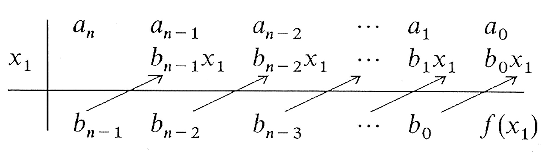
\includegraphics[width=6cm]{./bilder/Hornerschema_1.png}\\
$x_1 \Rightarrow$ Nullstelle (muss erraten werden!!)\\
oberste Zeile = zu zerlegendes Polynom
\end{minipage}
\begin{minipage}[t]{9cm}
\textbf{Beispiel:}\\
$f(x) = x^3-67x-126$\\
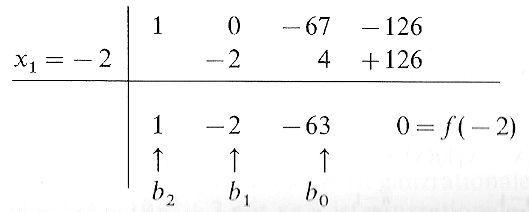
\includegraphics[width=6cm]{./bilder/Hornerschema_2.png}\\
$\Rightarrow f(x) = (x-x_1)(b_2x^2 + b_1x + b_0) = (x+2)(x^2-2x-63)$	
\end{minipage}

\subsection{Lineare Differentialgleichungssysteme erster Ordnung mit konstanten
Koeffizienten}
\begin{tabular}{p{8cm}p{8cm}}
\textbf{Form:}&
$\dot{x}=ax+by+f(t)$\\
&
$\dot{y}=cx+dy+g(t)$\\
\textbf{Die allgem. Lösung ergibt sich aus der DGL:}&
$\ddot{x}-(a+d)\dot{x}+(ad-bc)x=\dot{f}(t)-df(t)+bg(t)$\\
&
$y=\frac{1}{b}(\dot{x}-ax-f(t)))$\\
\end{tabular}

\end{document}
